\chapter{Background} \label{ch:background}

This chapter presents the background knowledge that the thesis builds upon. We start by introducing the various components of network delay, and follow up by presenting the main protocol used today for transmitting data on the Internet. The later sections goes into both somewhat old and more recent technologies that has emerged in order to improve the performance of Internet.









\section{Network Delay and Latency}

The time it takes for a bit of data to travel across the network from one communication endpoint to another is known as \textit{delay}. The process for such a transmission involves many components. A typical example where the data traverses an intermediate device before reaching destination follows. First, the data to be sent is usually created by an application. The data will then be handed over to the \gls{os} which passes it further down to the network interface card. From there, the data will be encoded and transmitted over a physical medium and eventually received by an intermediate device, such as a router. The router will then analyze the data and retransmit it over another medium that points to the destination. Finally, the data reaches the receiver. The whole process can happen in either multiples or fractions of seconds.

Network delay is therefore divided into the following four parts:

\begin{itemize}
    \item Processing delay --- time it takes a router to process the packet header
    \item Queuing delay --- time the packet spends in routing queues
    \item Transmission delay --- time it takes to push the packet's bits onto the link
    \item Propagation delay --- time for a signal to reach its destination
\end{itemize}

It is common to notify the sender that the receiver actually got the data. This is done by sending a signal from the receiver back to the sender, known as an \gls{ack}. The total time it takes for a sender to send data \textit{and} receive back an \gls{ack} is known as \textit{latency} or \gls{rtt}.

In this thesis, we are mainly concerned with the \textit{queuing} delay part.









\section{Transmission Control Protocol} \label{sec:tcp}

Whenever a user sends an email, or any data over the network for that matter, one should expect some kind of assurance that the delivery of the data was successful. This notion is known as \textit{reliability}, and is one of the key components of the \gls{tcp} and why it is one of the main protocols for transmitting data on the Internet. In essence, \gls{tcp} is a communication protocol that provides reliable, ordered, and error-checked delivery of data between applications such as \gls{www}, email and file transfer.

The main job of the \gls{tcp} is to package data into \textit{segments} or \textit{packets}, send them and then reassemble them on the receiving side. To ensure the reliability of these segments, a \textit{sequence number} is contained in each of them so that the receiver side can reassemble them in correct order. The sequence numbers also act as a safeguard when some packet has been lost, as the receiver will know what is missing. If the sender has not received an \gls{ack} within what is known as a \textit{timeout} interval, the missing data will be retransmitted.

Another distinguishing feature of \gls{tcp} is the notion of \textit{flow control}. Network devices have finite resources, and so some will be much faster than others. One device may be sending data at a much faster rate than the receiver can handle. \gls{tcp} solves this by using a \textit{sliding windows} mechanism which the sole purpose of controlling the flow of data between two devices such that one is not overwhelmed.









\subsection{Congestion Control} \label{sec:cc}

In the same sense that traffic on the road can come to a halt, the same is true for traffic on a network. This is known as \textit{congestion}, and is usually caused by overutilization. That is, network devices such as a router have finite resources, and thus too much traffic will cause the device to carry more data than it can handle which leads to congestion on the network. Typical effects include queueing delay, packet loss or the blocking of new connections.

The notion of congestion led to another key compononent of \gls{tcp}, which is the ability to either prevent congestion or mitigate it after it occurs. The means of applying \glsfirst{cc} is simple --- ensure that the sender does not overflow the network. In other words, the sender's rate needs to be adjusted based on the condition of the network. Now to the hard part --- how to adjust it?

To shed some light on this, \gls{tcp} includes a state variable called \gls{cwnd} which limits the amount of data that a sender can send before receiving an \gls{ack} back. This variable is known only to the sender, and serves as the key role for attaining \gls{cc}. The means of adjusting \gls{cwnd} is referred to as an \textit{congestion-control algorithm}, and consists of four intertwined parts:

\begin{itemize}
    \item Slow start --- gradually increase the amount of data transmitted until the capacity of the network has been reached.
    \item Congestion avoidance --- slowly probe for available bandwidth.
    \item Fast retransmit --- perform retransmission isntead of waiting for a timeout.
    \item Fast recovery --- enter congestion avoidance phase instead of slow start after a fast retransmit.
\end{itemize}

The following sections will describe each part in more detail.




\subsubsection{Slow Start and Congestion Avoidance}

Slow start and congestion avoidance are two independent algorithms with different objectives, but in practice are implemented together and so will be discussed together.

Upon a \gls{tcp} connection, the \gls{cwnd} value is initialized to a single \textit{segment} with a specified size. This size is either  announced by the the other end, known as the \gls{rwnd}, or set to a typical default \cite{rfc5681}. In the same sense that \gls{cwnd} is a sender-side limit, \gls{rwnd} is a receiver-side limit. Together, the minimum of \gls{cwnd} and \gls{rwnd} governs the data transmission in slow start. However, at the beginning of a transmission, the network conditions are unknown, so the goal of the slow start phase is simple --- slowly probe the network to determine the available capacity.

To find the capacity, slow start works as follows --- the sender starts by transmitting one segment. For every received \gls{ack}, increment the \gls{cwnd} by another segment, effectively doubling it every \gls{rtt}. Repeat this process until a timeout occurs. That is, until the capacity has been reached that is signaled by a router starting to drop packets, which tells the sender that its \gls{cwnd} has grown too large.

As a response to hitting the threshold, \gls{tcp} will now halve the \gls{cwnd} since that is the last known value to not induce a timeout. This new value is known as the \gls{ssthresh}, and is another \gls{tcp} state variable used to determine whether the slow start or congestion avoidance algorithm is used to control the data transmission. In other words, the slow start phase ends when \gls{cwnd} reaches or exceeds \gls{ssthresh}.

The goal of congestion avoidance is also simple --- avoid congestion, as the name implies. But the challenge here is to maintain a transmission rate that it not too low, otherwise the link becomes underutilized, and at the same time probe for available bandwidth without overflowing the network too quickly. To do so, a feedback control algorithm known as \gls{aimd} is used.

Let $w(t)$ be the sending rate during time slot $t$, let $a$ be a positive number and $b$ a number between $0$ and $1$. The sending rate can then be modeled as \gls{aimd} by

\begin{equation} \label{eq:aimd}
    w(t + 1) = \begin{cases}
        w(t) + a, & \text{if congestion is not detected},\\
        w(t) \times b, & \text{if congestion is detected}.
    \end{cases}
\end{equation}

where $a$ is the additive increase factor, and $b$ is the multiplicative decrease factor.

\begin{figure}[H]
    \centering
    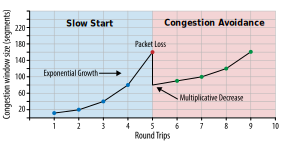
\includegraphics[width=0.7\textwidth]{TCP_Congestion_Control_Simple}
    \captionsetup{width=0.7\textwidth}
    \caption{The two main parts of \gls{cc} --- the slow start phase where \gls{cwnd} grows exponentially, and the congestion avoidance phase where the transmission rate is increased more conservatively. (\href{https://hpbn.co/building-blocks-of-tcp/}{\textit{source}})}
\end{figure}

\gls{aimd} provides linear growth of the \gls{cwnd} when probing for available bandwidth, and a multiplicative reduction when congestion is detected.









\subsubsection{Fast Retransmit and Fast Recovery}

Fast retransmit and fast recovery are two algorithms that aims to speed up the recovery process of a \gls{tcp} connection in the event of a segment loss, but without re-entering the slow start phase. As with slow start and congestion avoidance, both are in practice implemented together and so will be discussed together.

In a \gls{tcp} connection, the sender uses a simple timer to recognize lost segments. That is, if an \gls{ack} is not received within a specified time, the sender will assume that the segment has been lost and so will retransmit it. Fast retransmit is an enhancement to \gls{tcp} that reduces the time a sender waits before retransmitting a lost segment. The duration is determined by the amount of duplicate \gls{ack}s, which the receiver will keep sending to indicate the next expected sequence number. Generally, if only one or two duplicate \gls{ack}s are experienced, it is assumed that a simple reordering of the segments will solve the problem. But when three or more duplicate \gls{ack}s are received in a row, it signals a strong indication that a segment has been lost. In such a case, \gls{tcp} will perform a retransmission instead of waiting for a timeout, known as a \textit{fast transmit}.

When a fast retransmit has occured, the sender will transmit what appears to be the missing segment. However, the slow start phase will not be performed after this, but rather the congestion avoidance phase. This is known as the \textit{fast recovery} algorithm. Since only a segment seems to be missing, it would be wasteful to redue the traffic flow abruptly by going into slow start. Instead, a fast recovery is initiated, allowing for sustained high throughput under moderate congestion.

\begin{figure}[H]
    \centering
    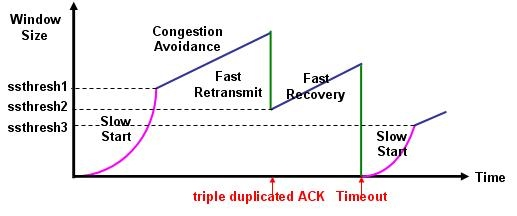
\includegraphics[width=0.6\textwidth]{TCP_Congestion_Control_Complete}
    \captionsetup{width=0.6\textwidth}
    \caption{A more complete illustration of a congestion-control algorithm including all four parts --- slow start, congestion avoidance, fast retransmit and fast recovery. (\href{https://sites.google.com/site/projectcodebank/computer-engineering-notes/tcp-congestion-control-algorithm}{\textit{source}})}
\end{figure}






\subsection{Bufferbloat}

It is easy to fall into the trap of believing that bigger buffers would increase network performance. After all, why drop a packet when you can avoid it by a buffer that never gets full in the first place. Likewise, it is easy to see why a big buffer is bad --- it takes time to drain the queue. If more packets come in than can be transmitted, the longer the queue gets. As a result, the latency spikes. Excess buffering of packets is referred to as \textit{bufferbloat}, causing high latency and reducing the overall network throughput.

Still, some buffering is clearly needed so that a short burst of packets can be absorbed without significant loss. But how much? Ideally, for a particular network, we would want to keep the bottleneck link as busy as possible. A widely used formula in determining the buffer size $B$ is the \gls{bdp} \cite{sizing_router_buffers}:

\begin{equation}
    B = RTT_{avg} \times C
\end{equation}

where $RTT_{avg}$ is the average \gls{rtt} of the flow passing through the link and $C$ is the capacity of the link. However, if the average \gls{rtt} is relatively high such as \SI{250}{ms} and a router has a Gigabit Ethernet interface, then the buffer size would at least be $B = \SI{250}{\milli\second} \times \SI{1}{\giga\bit} = \SI{32}{\mega\byte}$. Such large buffers have been shown to greatly contribute to the bufferbloat problem, especially on backbone routers that uses slow, off-chip DRAMs. Nick McKeown et. al. from \cite{sizing_router_buffers} showed that dividing the \gls{bdp} by the square root of number of flows yielded a radical better estimate for buffer sizing, so far as a 99\% reduction in buffer size with negligible difference in throughput. In other words, the better formula for estimating the buffer size is then

\begin{equation}
    B = \frac{RTT_{avg} \times C}{\sqrt{n}}
\end{equation}

where $n$ is the amount of flows on a given link.




\subsection{TCP Variants}

The two first \gls{tcp} \gls{cc} algorithms that became widely used was called Tahoe and Reno. Both uses packet loss as a congestion signal, and both react by halving their \gls{cwnd}. With the increase in network speeds, other loss-based algorithms were proposed. One of these were called NewReno, which improved the retransmission during the fast recovery phase of Reno. NewReno became widely popular, and is currently the default \gls{cc} algorithm used on FreeBSD today. NewReno follows the behavior described in Section \ref{sec:cc} and produces the classical \textit{sawtooth} pattern shown in the following Figure \ref{fig:newreno}.

\begin{figure}[H]
    \centering
    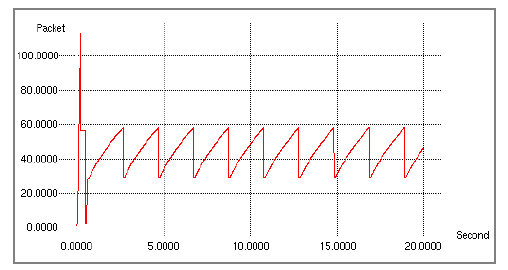
\includegraphics[width=0.5\textwidth]{TCP_CC_NewReno}
    \captionsetup{width=0.5\linewidth}
    \caption{The classic \textit{sawtooth} pattern of \gls{cwnd} over time using the \gls{tcp} congestion control algorithm NewReno.}
    \label{fig:newreno}
\end{figure}

Another \gls{cc} algorithm that became popular was CUBIC, aiming to optimize the congestion control in high bandwidth networks with high latency. CUBIC was implemented and used by default in Linux kernel versions 2.6.19 and above, which persists to this day. As its name implies, CUBIC does not use a linear function to adjust its \gls{cwnd}, but rather a cubic function as shown in the following Figure \ref{fig:cubic}.

\begin{figure}[H]
    \centering
    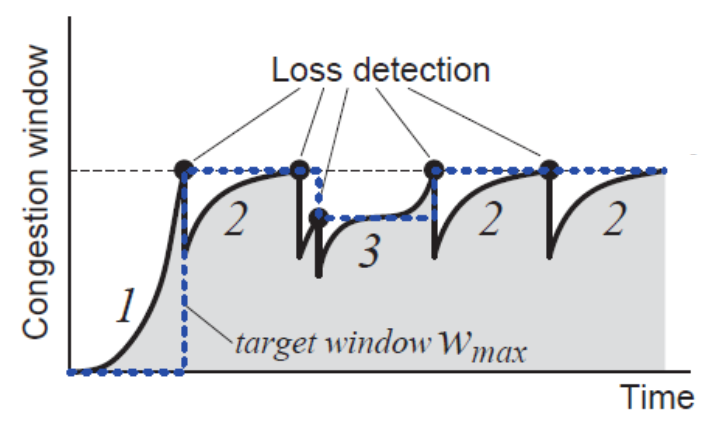
\includegraphics[width=0.4\textwidth]{cubic}
    \captionsetup{width=0.4\linewidth}
    \caption{The behavior of the CUBIC congestion control algorithm.}
    \label{fig:cubic}
\end{figure}




\section{Active Queue Management}

When a packet arrives at the incoming port of a router, it is often the case that there is not enough memory to buffer it, and so an important decision must be made --- should the newly arrived packet simply be dropped, or should one of the already-queued packets be dropped to make room for the new one? In the early days of networking, the queue management algorithm called \textit{tail drop} was used, simply dropping newly arrived packets when the queue was filled. However, this approach is considered unfair among traffic flow due to its \textit{first come, first serve} basis, leaving little room for new participants since a single connection could monopolize the queue space. \cite{on_traffic_phase_effects_in_packet_switched_gateways} Tail drop also lead to what is known as \textit{\gls{tcp} global synchronization}, where all connections would both simultaneously "hold back" and then step forward, causing networks to become underutilized and flooded in alternate waves.

Over the years, many new suggestions and algorithms were made. They collectively became known as \glsfirst{aqm} algorithms --- the policy of dropping packets \textit{before} a buffer becomes full. One of the first and most widely implemented algorithm to surface was \gls{red}, addressing the issues of tail drop. By preemptively dropping packets \textit{probabilistically} before the buffer became full, \gls{red} would avoid both global synchronization and the problem of new bursty connections being penalized. \cite{ieee251892}

Widespread usage of \gls{red} also revealed a core problem --- it was difficult to configure, requiring complex fine-tuning in order to achieve significant performance gains. Variants of \gls{red} were developed to accommodate for this, such as BLUE, and later many new \gls{aqm} schemes. A few selected will be discussed briefly in the next sections.



\subsection{Controlled Delay}

\gls{codel} is a more recent \gls{aqm} scheme developed by Van Jacobsen. It is designed to overcome bufferbloat in modern networking environments by limiting, or \textit{controlling}, the delay that network packets experience when passed through buffers in networking hardware. An implementation of \gls{codel} for the Linux kernel was written in 2012 by Dave Täht and Eric Dumazet. It has since been adopted as the standard \gls{aqm} for the widely known OpenWrt \gls{os} used by many routers.

Van Jacobsen himself asserted in 2006 that existing \gls{aqm}s have been using incorrect means of recognizing bufferbloat. \cite{a_rant_on_queues} Algorithms such as \gls{red} measures the average queue length and considers it a case of bufferbloat if the average grows too large. Jacobsen demonstrated in 2006 that this is not necessarily the case, as a quick burst also exhibits the same behaviour. In fact, Jacobsen would say that queue length was no indicator at all about packet demand or network load, \cite{a_rant_on_queues, controlling_queue_delay} suggesting instead that the minimum queue length during a sliding time window would be a better metric. \cite{controlling_queue_delay}

Jacobsen would therefore properly combat bufferfloat in \gls{codel} by distinguishing between two types of queue --- a \textit{good} queue that exhibits no bufferbloat, and a \textit{bad} queue that actually exhibits bufferbloat. The \gls{codel} approach, in summary, is designed to meet the following goals: \cite{rfc8289}

\begin{itemize}
    \item Make \gls{aqm} parameterless for normal operation.
    \item Be able to distinguish a good queue from a bad one in order to keep delay low while allowing necessary bursts of traffic.
    \item Control delay while insensitive to \gls{rtt} delays, link rates, and traffic loads --- all without harming the network.
    \item Adapt to dynamically changing link rates with no negative impact on utilization.
    \item Allow simple and efficient implementation.
\end{itemize}





\subsection{Proportional Integral Controller Enhanced}

\gls{pie} is another recent \gls{aqm} algorithm to control queuing latency directly in order to address the bufferbloat problem. It was made by a group of authors from Cisco Systems as a lightweight alternative to \gls{codel}, claiming that \gls{codel} cannot practically be implemented in hardware --- first, \gls{codel} requires packets to be timestamped when enqueued, and second, the drop decision happens on dequeue, so all packets have to be queued. \gls{pie}, on the other hand, performs the drop decision on enqueue, similar to \gls{red} and most other \gls{aqm} schemes. Hence, \gls{pie} incurs very little overhead and is simple enough to implement in both hardware and software.

The \gls{pie} approach, much like \gls{codel}, is designed to meet the following goals: \cite{rfc8033}

\begin{itemize}
    \item Control queuing latency instead of queue length to combat bufferbloat.
    \item Attaining a delicate balance between high link utilization and low latency.
    \item Simple to implement and easily scalable in both hardware and software by striving to maintain similarity to that of \gls{red}.
    \item Ensure system stability for various network topologies and scale well across an arbitrary number of streams.
    \item Design parameters should be set automatically. Users only need to set performance-related parameters such as target queue latency, not design parameters.
\end{itemize}







\section{Explicit Congestion Notification}

Conventially, the means of detecting network congestion has been by packet loss or a long enough delay inducing a timeout. Then the addition of \gls{aqm} came to the Internet infrastructure, adding the ability for routers to detect congestion before the queue overflows. Both loss and delay are \textit{implicit} signals of congestion, and in 2001, an extension to \gls{tcp} and \gls{ip} was defined \cite{rfc3168} to allow for \textit{explicit} congestion signaling --- called \gls{ecn} --- enabling end-to-end notification of network congestion without dropping packets.

\begin{wraptable}{r}{9cm}
    \begin{tabular}{|c|l|l|}
        \multicolumn{3}{c}{ECN Code Points} \\
        \hline
        Code & Description & Shorthand \\
        \hline
        00 & Non ECN-Capable Transport & Non-ECT \\
        \hline
        01 & ECN Capable Transport & ECT(0) \\
        \hline
        10 & ECN Capable Transport & ECT(1) \\
        \hline
        11 & Congestion Encountered & CE \\
        \hline
    \end{tabular}
    \caption{The four different code points for \gls{ecn} that is encoded in the \gls{ip} header.}
    \label{table:ecn}
\end{wraptable}

\gls{ecn} is a form of network-assisted \gls{cc}, meaning that the entire underlying network infrastructure must support it. For this to work, the new \gls{ecn} mechanism consists of two components:

\begin{itemize}
    \item Two new bits has been added to the \gls{ip} header in order to explicitly communicate \gls{ecn}-capability and indication of congestion on the network (see table \ref{table:ecn}).
    \item Two new flags has been added to the \gls{tcp} header --- the \gls{ece} flag so that the receiver can inform a sender when a \gls{ce} packet has been received, and the \gls{cwr} flag so that a sender can inform the receiver that the \gls{cwnd} has been reduced.
\end{itemize}

An \gls{ecn}-capable network works as follows. A sender will transmit \gls{ip} packets with either the \gls{ect}(0) or \gls{ect}(1) bit set. Then, when there is congestion, a router (in conjuction with \gls{aqm}) will start marking the packets by setting the \gls{ce} bit. The receiver will then see this, and echo back the congestion indication to the sender with an \gls{ece} packet. The sender will then reduce its \gls{cwnd} value and respond with an \gls{cwr} packet.

\gls{ecn} was standardized in 2001 as a direct replacement for the use of packet loss as congestion signaling. \cite{rfc3168} Despite its positive early impact \cite{rfc2884}, it never saw widespread usage. \cite{enabling_internet-wide_ecn} A series of unfortunate incidents managed to cripple its early deployment --- rather than responding properly or ignoring the \gls{ecn} bits, some firewalls on faulty network equipment would instead block or mangle packets with \gls{ecn} bits set. This incorrect behaviour led to failure rate of 8\% in \gls{ecn}-enabled \gls{tcp} connections for web servers tested in 2004. \cite{pre-congestion_notification}

Due to the unfortunate early struggles of \gls{ecn} deployment, the \gls{ietf} required that the response to an \gls{ecn} signal should be the same as the reaction to a loss. \cite{rfc3168} However, this requirement has recently been relaxed, \cite{rfc8311} sparking a regained interest in the field and giving rise to new experimental \gls{ecn} proposals. As of 2015, measurements show that the failure of \gls{ecn}-enabled \gls{tcp} connections has reduced to less than 1\%. \cite{enabling_internet-wide_ecn}





\section{Alternative Backoff with ECN}

\glsfirst{abe} \cite{abe} is a recent proposal utilizing \gls{ecn} in congestion control. It is a simple sender-side only modification that can be summarized as follows:

\begin{itemize}
    \item Upon a packet loss, a \gls{tcp} sender should reduce its \gls{cwnd} as usual (e.g. 50\% with NewReno or 30\% with CUBIC).
    \item Upon the receipt of an \gls{ecn} mark, a \gls{tcp} sender should reduce \textit{less} than the usual response for loss.
\end{itemize}

The less aggressive multiplicative decrease factor yielded significant performance gains in lightly-multiplexed scenarios. Specifically, a 20\% reduction factor was found to give a good latency-vs-utilization trade-off.

As of 2018, \gls{abe} has been formalized by the \gls{ietf} as an experimental \gls{rfc} \cite{rfc8511} and been implemented in mainline FreeBSD \gls{os} kernel.
